\section{Architectural Overview}\label{sec:arch}

The basic architecture to develop the system outlined above will consist of the following parts:

\begin{itemize}
\item The smartphone, including a NFC chip as well as an internet connection to register with the service. The internet connection will be needed only one time to initialize the system or to negotiate a new key in case of revocation.
\item The Door Access System, also including a NFC chip which can send and receive. A simple NFC reader would not be enough due to simple replay attacks. The Door Access System also needs access to the internet or at least to an intranet to check if the student or the employee has access to the specific area and to get other information for realizing security features like encryption of the communication. Therefore, some kind of computer is needed, interacting with the NFC hardware as well as with the back-end.
\item A back-end system, which will take care of key generation and storage in case of a public-key system or other sensitive data like hash values.

\item The TUMOnline system since is in the possession of the enrollment information of every student.
\end{itemize} 
%
A basic overview of the overall architecture (based on public-key cryptography as discussed in section \ref{sec:alt:proto:pubkey}): \newline
 \begin{center}
	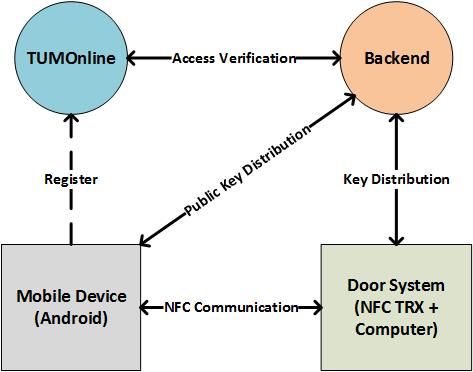
\includegraphics[scale=0.8]{basic_architecture.jpg}
\end{center}


\subsection{Registration with Back-end}
To initialize the system, the user has to contact the back-end system once for authentication by providing its user ID.
To activate the user token that is generated by TUMOnline, the user has to login separately in its web platform. 
The back-end system can check if the proposed access token of the user is valid or not through TUMOnline Webservice API.
%For that purpose, the connection to the TUMOnline service is needed to get this kind of information.
If the user has sent the right access token, the back-end system will create a public key pair and will send the user his private key. Therefore, a key storage and management system has to be implemented.
All connections to the back-end are planned to be secured by TLS.


\subsection{Authentication between Smartphone and NFC Transceiver}
After the user has registered with the back-end system, he can communicate with the NFC reader. 
A three-way handshake assures a secure connection between smartphone and NFC reader.
In order to verify the soundness of the procedure, in particular the authenticity of the communication partner, the NFC reader (i.e.~the system behind it) will fetch the public key of the user who wants to authenticate from the back-end system.
Further, the Door Access System will check if the user has access to the requested area.
It will finally unlock the door if all checks were positive.
